\documentclass[tikz,border=8pt]{standalone}
% Shared look for every TikZ diagram. Load with % Shared look for every TikZ diagram. Load with % Shared look for every TikZ diagram. Load with \input{../../tools/tikz-style.tex}
\usepackage[T1]{fontenc}
\usepackage{lmodern}
\renewcommand{\sfdefault}{lmr}  % diagrams use the same serif as the text
\usetikzlibrary{arrows.meta, positioning, shapes.geometric, calc, fit, backgrounds}
\definecolor{cblue}{HTML}{4C78A8}
\definecolor{corange}{HTML}{F58518}
\definecolor{cgreen}{HTML}{54A24B}
\definecolor{cred}{HTML}{E45756}
\definecolor{cpurple}{HTML}{B279A2}
\definecolor{cgrey}{HTML}{6B6B6B}
\tikzset{
  every picture/.style={font=\sffamily, line width=1.2pt},
  box/.style={draw=#1, fill=#1!12, rounded corners=4pt, align=center, inner sep=7pt, minimum height=1.1cm},
  box/.default=cgrey,
  arrow/.style={-{Stealth[length=3mm]}, draw=cgrey, line width=1.4pt},
  title/.style={font=\sffamily\bfseries\Large},
  note/.style={font=\sffamily\small, text=cgrey, align=center},
}
\AtBeginDocument{\hyphenpenalty=10000 \exhyphenpenalty=10000}

\usepackage[T1]{fontenc}
\usepackage{lmodern}
\renewcommand{\sfdefault}{lmr}  % diagrams use the same serif as the text
\usetikzlibrary{arrows.meta, positioning, shapes.geometric, calc, fit, backgrounds}
\definecolor{cblue}{HTML}{4C78A8}
\definecolor{corange}{HTML}{F58518}
\definecolor{cgreen}{HTML}{54A24B}
\definecolor{cred}{HTML}{E45756}
\definecolor{cpurple}{HTML}{B279A2}
\definecolor{cgrey}{HTML}{6B6B6B}
\tikzset{
  every picture/.style={font=\sffamily, line width=1.2pt},
  box/.style={draw=#1, fill=#1!12, rounded corners=4pt, align=center, inner sep=7pt, minimum height=1.1cm},
  box/.default=cgrey,
  arrow/.style={-{Stealth[length=3mm]}, draw=cgrey, line width=1.4pt},
  title/.style={font=\sffamily\bfseries\Large},
  note/.style={font=\sffamily\small, text=cgrey, align=center},
}
\AtBeginDocument{\hyphenpenalty=10000 \exhyphenpenalty=10000}

\usepackage[T1]{fontenc}
\usepackage{lmodern}
\renewcommand{\sfdefault}{lmr}  % diagrams use the same serif as the text
\usetikzlibrary{arrows.meta, positioning, shapes.geometric, calc, fit, backgrounds}
\definecolor{cblue}{HTML}{4C78A8}
\definecolor{corange}{HTML}{F58518}
\definecolor{cgreen}{HTML}{54A24B}
\definecolor{cred}{HTML}{E45756}
\definecolor{cpurple}{HTML}{B279A2}
\definecolor{cgrey}{HTML}{6B6B6B}
\tikzset{
  every picture/.style={font=\sffamily, line width=1.2pt},
  box/.style={draw=#1, fill=#1!12, rounded corners=4pt, align=center, inner sep=7pt, minimum height=1.1cm},
  box/.default=cgrey,
  arrow/.style={-{Stealth[length=3mm]}, draw=cgrey, line width=1.4pt},
  title/.style={font=\sffamily\bfseries\Large},
  note/.style={font=\sffamily\small, text=cgrey, align=center},
}
\AtBeginDocument{\hyphenpenalty=10000 \exhyphenpenalty=10000}

\begin{document}
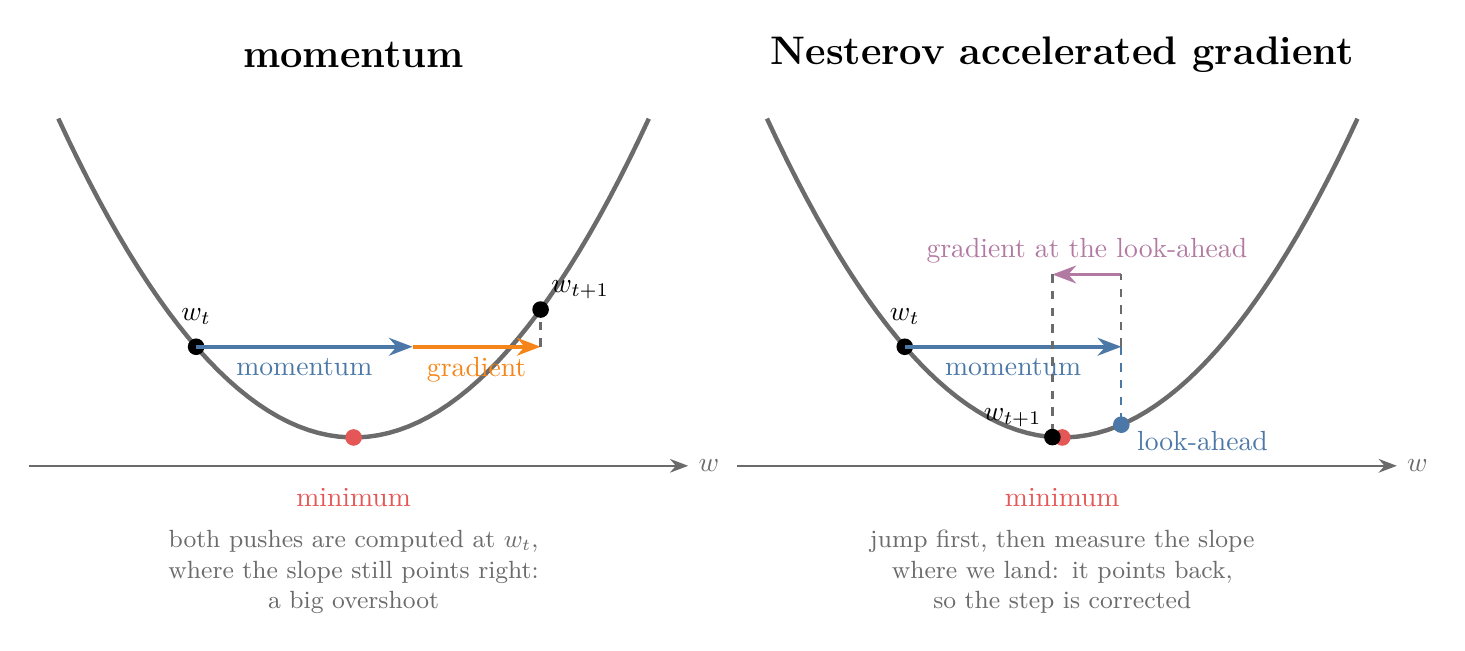
\begin{tikzpicture}[every node/.append style={font=\sffamily}, x=1.25cm, y=0.9cm]
  % ---------- left: momentum ----------
  \begin{scope}
    \node[title] at (0,5.4) {momentum};
    \draw[cgrey, line width=1.6pt, domain=-3:3, samples=60] plot (\x, {0.5*\x*\x});
    \draw[-{Stealth}, cgrey, line width=0.8pt] (-3.3,-0.4) -- (3.4,-0.4) node[right] {$w$};
    \fill[cred] (0,0) circle (3pt); \node[text=cred] at (0,-0.85) {minimum};
    \fill[black] (-1.6,1.28) circle (3pt) node[above=4pt] {$w_t$};
    % momentum jump and gradient step, both from w_t
    \draw[arrow, draw=cblue] (-1.6,1.28) -- node[below, text=cblue] {momentum} (0.6,1.28);
    \draw[arrow, draw=corange] (0.6,1.28) -- node[below, text=corange] {gradient} (1.9,1.28);
    \draw[dashed, cgrey, line width=0.8pt] (1.9,1.28) -- (1.9,1.805);
    \fill[black] (1.9,1.805) circle (3pt) node[above right] {$w_{t+1}$};
    \node[note, text width=5.6cm] at (0,-1.9) {both pushes are computed at $w_t$,\\where the slope still points right:\\a big overshoot};
  \end{scope}
  % ---------- right: NAG ----------
  \begin{scope}[xshift=9.0cm]
    \node[title] at (0,5.4) {Nesterov accelerated gradient};
    \draw[cgrey, line width=1.6pt, domain=-3:3, samples=60] plot (\x, {0.5*\x*\x});
    \draw[-{Stealth}, cgrey, line width=0.8pt] (-3.3,-0.4) -- (3.4,-0.4) node[right] {$w$};
    \fill[cred] (0,0) circle (3pt); \node[text=cred] at (0,-0.85) {minimum};
    \fill[black] (-1.6,1.28) circle (3pt) node[above=4pt] {$w_t$};
    \draw[arrow, draw=cblue] (-1.6,1.28) -- node[below, text=cblue] {momentum} (0.6,1.28);
    \fill[cblue] (0.6,0.18) circle (3pt);
    \draw[dashed, cblue, line width=0.8pt] (0.6,1.28) -- (0.6,0.18);
    \node[text=cblue, right] at (0.65,-0.05) {look-ahead};
    \draw[arrow, draw=cpurple] (0.6,2.3) -- node[above, text=cpurple] {gradient at the look-ahead} (-0.1,2.3);
    \draw[dashed, cgrey, line width=0.8pt] (0.6,1.28) -- (0.6,2.3);
    \draw[dashed, cgrey, line width=0.8pt] (-0.1,2.3) -- (-0.1,0.005);
    \fill[black] (-0.1,0.005) circle (3pt);
    \node[above left] at (-0.1,0.0) {$w_{t+1}$};
    \node[note, text width=5.6cm] at (0,-1.9) {jump first, then measure the slope\\where we land: it points back,\\so the step is corrected};
  \end{scope}
\end{tikzpicture}
\end{document}
